%------------------
\section{Tree Search Algorithm\label{sec:ch2:treesearch}}

With a better understanding of the colored graph isomorphism problem in the context of architecture design, a tree search algorithm was developed to more efficiently enumerate a graph structure space that contains $\mathcal{G}_3$. This algorithm is based on the idea that for simple components, the port ordering does not matter so we are free to always choose the first port of a component when making edges.
 
Algorithm~\ref{alg:ch2:simpletree} starts with a vector for length $N_C$ where the entries are the number of ports for every component in $G^{CC}$. For example, if $P = [1\ 2]$ and $R=[2\ 3]$, then this vector would be $\xvar{V} = [1\ 1\ 2\ 2\ 2]$ and $\xvar{cVf} = [2\ 3\ 5\ 7\ 9]$. Recursion is then applied to enumerate all possible edge combinations where each recursive step adds an edge. The end result is a set of missorted \mypm{}s, i.e.,~the sequential pairs that define the edges need to be sorted such that they fit the definition of a \mypm{} in Sec.~\ref{sec:ch2:inter} (but no \mypm{} will occur twice and the property of naturally satisfying \ref{ch2:s2} and \ref{ch2:s6} is maintained). The end result is an algorithm that does not produce many \mypm{} graphs that would certainly have a port-type isomorphism. A visualization of the tree-like behavior is in Fig.~\ref{fig:ch2:tree1simple} where each leaf in the tree is a new call of the algorithm and the branches are the loops through the possible remaining edges. Not all leaves have the same number of branches since components become completely connected at different times. Two paths are shown in the figure for a particular architecture design problem, each resulting in a different \mypm{}. Note that the thicker black lines indicate the chosen edge and the gray lines are the other potential edges for the particular leaf instance.

\begin{figure}
\centering
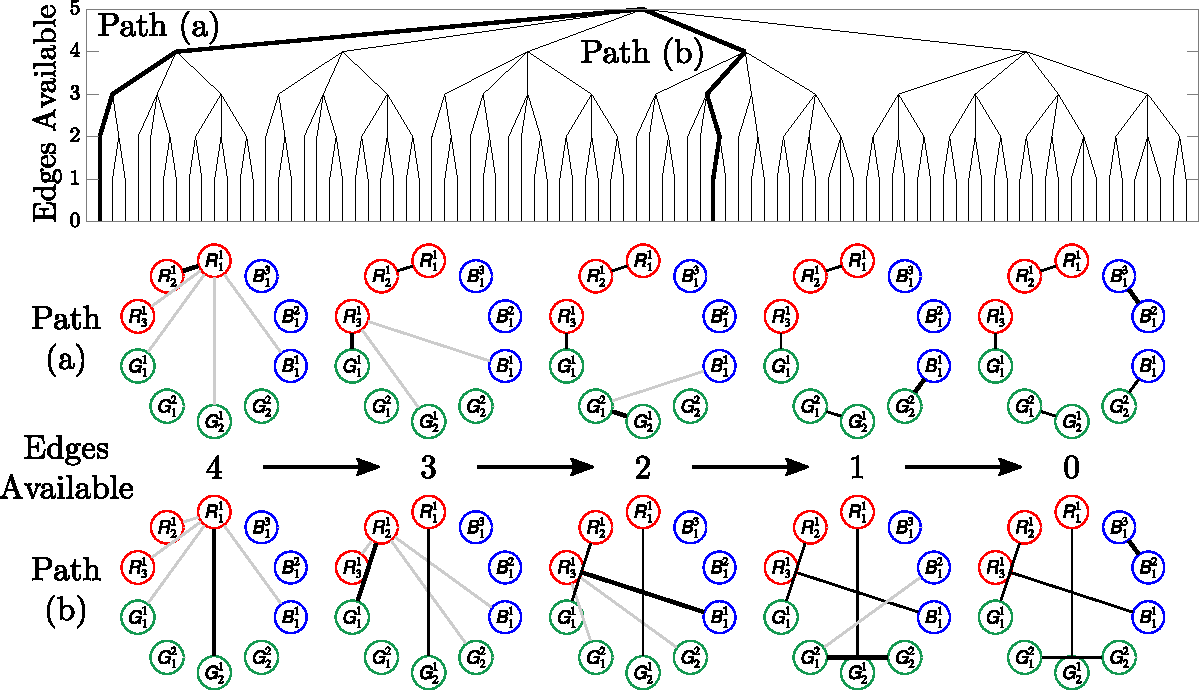
\includegraphics[width=\columnwidth]{../ch2/figures/tree1simple_optimized}
\caption[Tree structure for \nameref{sec:ch2:example1} using the basic tree search algorithm]{Tree structure for \nameref{sec:ch2:example1} using the basic tree search algorithm in Alg.~\ref{alg:ch2:simpletree}.\label{fig:ch2:tree1simple}}
\end{figure}

This approach is similar to a number of reported graph enumeration algorithms \cite{Carhart1975a, Colbourn1979a, Snavely1993a, Faulon2003b}.
The tree algorithm shares some similarities with deletion orderly algorithms \cite{Colbourn1979a}.
Snavely and Papalambros developed a tree algorithm that only deals with structured components, which limits the design space by the number of components rather than the $(C,R,P)$ notation in this work \cite{Snavely1993a}. 
Faulon et al. enumerate molecules of a specific signature height with a recursive algorithm, but do not allow for components to be removed. Thus, they do not cover the same architecture design space \cite{Faulon2003b}. 
Neither of these works make the connection between \mypm{} theory and architecture enumeration which provides a number of insights and practical functions. 

We can further improve on this algorithm by adding a single line between lines~\ref{ch2:line3} and \ref{ch2:line4} that will result in graphs that always satisfy \ref{ch2:s5} (feasible edge constraints). First, expand $A_R$ such that its size is the same as $G^{CC}$ where 0 entries still indicate infeasible edge constraints. The additional line would then be: $\xvar{Vallow}$ $\leftarrow$  $\xvar{A}(\xvar{iL},:) \circ \xvar{V}$. By finding the nonzero entries of $\xvar{Vallow}$ instead of $\xvar{V}$, we limit the for-loop to edges that are feasible. This has the intentional effect that certain branches of the tree will terminate before a feasible \mypm{} is found. Therefore when \ref{ch2:s5} is present, we will utilize this `improved' tree search algorithm to more efficiently enumerate $\mathcal{G}_3$.
Additional enhancements to the tree search algorithm are discussed in Appendix~\ref{app:A} as well as alternative tree traversal strategies.

% \IncMargin{1em}
\RestyleAlgo{algoruled}

\begin{vAlgorithm}[t]{\columnwidth}{0em}

\LinesNumbered
\SetSideCommentRight 
\DontPrintSemicolon
% \SetNoFillComment

% \SetTitleSty{\textsf}{small}
% \renewcommand{\algorithmcfname}{\small\textbf{\textsf{\MakeUppercase{Algorithm}}}}%

% \SetKwData{Left}{left}\SetKwData{This}{this}\SetKwData{Up}{up}
\SetKwFunction{cumprod}{cumprod}
\SetKwFunction{length}{length}
\SetKwFunction{zeros}{zeros}
\SetKwFunction{ceil}{ceil}
\SetKwFunction{mod}{mod}
\SetKwFunction{mymin}{min}
\SetKwFunction{find}{find}
\SetKwFunction{detectiso}{isomorphic\_vf2}

\SetKwInOut{Input}{Input}
\SetKwInOut{Output}{Output}

\caption{Basic tree search algorithm. \label{alg:ch2:simpletree}}

\Input{$\xvar{V}$ -- vector of remaining ports for each component replicate \\
$\xvar{E}$ -- vector of edges in sequential pairs, initially empty \\
$\xvar{cVf}$ -- cumulative sum of the original $\xvar{V}$ plus 1 \\
$\xvar{SavedGraphs}$ -- set of graphs, initially empty \\
}
\Output{$\xvar{SavedGraphs}$ -- set of graphs \\
}
\BlankLine
            
    $\xvar{iL}$ $\leftarrow$  $\find(\xvar{V},\xvar{first})$ \tcc*{find first nonzero entry}
    
    $\xvar{L}$ $\leftarrow$  $\xvar{cVf}(\xvar{iL})-\xvar{V}(\xvar{iL})$ \tcc*{left port}
    
    $\xvar{V}\big(\xvar{I}(1)\big)$ $\leftarrow$ $\xvar{V}(\xvar{iL}) - 1$ \tcc*{remove port \label{ch2:line3}}
    
% \SetSideCommentLeft 
  %   \tcc*{$\xvar{V}$ $\leftarrow$  $\xvar{A}(\xvar{I}(1),:) \circ \xvar{V}$, naturally enforce \ref{ch2:s5} by using a potential adjacency matrix $\xvar{A}$}
% \SetSideCommentRight   
            
    $\xvar{I}$ $\leftarrow$  $\find(\xvar{V})$ \tcc*{find nonzero entries \label{ch2:line4}}  
    
	\For(\tcc*[f]{loop through all nonzero entries}){$\xvar{iR}\leftarrow$ $\xvar{I}$ \label{alg:ch2:cip:5} }{
	
        $\xvar{R}$ $\leftarrow$ $\xvar{cVf}(\xvar{iR})-\xvar{V}(\xvar{iR})$ \tcc*{right port}

        $\xvar{E2}$ $\leftarrow$ $[\xvar{E},\xvar{L},\xvar{R}]$ \tcc*{combine left, right ports for an edge }

		$\xvar{V2}$ $\leftarrow$ $\xvar{V}$ \tcc*{local remaining ports vector}
       
		% $\xvar{Eo}$ $\leftarrow$ $\xvar{E}$
               
        $\xvar{V2}(\xvar{iR})$ $\leftarrow$ $\xvar{V2}(\xvar{iR})-1$ \tcc*{remove port (local copy)}
	
		\uIf(\tcc*[f]{recursive call if any remaining vertices}){any element of $\xvar{V2}$ is nonzero}{
		
            $\xvar{SavedGraphs}$ $\leftarrow$ Algorithm~\ref{alg:ch2:simpletree} with $\xvar{V2},\xvar{E2},\xvar{cVf},\xvar{SavedGraphs}$
            
        }
        	
        \Else{
        	
            % $\xvar{id}$  $\leftarrow$ $\xvar{id}+1$ \tcc*{increment index of total graphs}
            
            $\xvar{SavedGraphs}\{\xvar{end} + 1\}$  $\leftarrow$ $\xvar{E2}$ \tcc*{save missorted perfect matching }
        	
        }
	
	} % end for i

\end{vAlgorithm}